\documentclass[11pt,a4paper]{article}
\usepackage{cite,url,hyperref,graphicx, amsmath, bm}
\usepackage{alltt} 
\usepackage{listings}
\usepackage{algorithm2e} % need texlive-science which I'm having trouble with getting...
\lstset{
basicstyle=\small\ttfamily,
columns=flexible,
breaklines=true
}



\setlength{\textwidth}{6.5in}
\setlength{\oddsidemargin}{0in}
\setlength{\evensidemargin}{0in}
\setlength{\topmargin}{-0.5in}
\setlength{\textheight}{25cm}
%opening
\title{Error Analysis of PSMC'}
\author{Alex Lee Jackson}
\begin{document}

\maketitle

%\begin{abstract}
%blah
%
%\end{abstract}
\section{Miscellaneous}
For further inquiries, I can be contacted at \href{mailto:aj123@internode.on.net}{aj123@internode.on.net}, or DM'd on the \texttt{rstat} Slack.

GitHub: \url{https://github.com/alex-jackson1994/errorAnalysis}

\section{Objective}
Determine if there's a relationship between the lengths of contigs being analysed, population model (predictors) and the error (response) given by PSMC' (MSMC\cite{schiffels2014inferring} with two haplotypes). This will probably be done using mixed effects models.\\

\begin{algorithm}[H]
  \For{Each population model (3)}{
    \For{Each simulated genome (5)}{
      \For{Each model of fragmentation (2)}{
        \For{Each level of fragmentation (5)}{
          Run MSMC, record output.\
        }
      }
    }
  }
  \caption{Outline of the simulation and MSMC analysis process}\label{overall}
\end{algorithm}

\subsection{Background}
PSMC' gives an estimate of how population demographics change over time, by analysing heterozygousity of sites across a genome. However, real sequenced genomes will not always be nicely sorted into chromosomes. Often they will be assembled into smaller sections called contigs. We will simulate human genomes (MSMC was originally written to analyse humans) under the following conditions:
\begin{itemize}
\item The length $L$ of the genome will be taken from a real human genome. For simplicity, \emph{only autosomes} will be considered.
\item Three different population models will be considered. Take time $t$ as going from recent to ancient, i.e. $t=0$ is the more recent than $t=100$. These dynamics should be carefully considered, as we want them to fall into the time range where PSMC' can actually pick them up.
\begin{itemize}
\item Constant: $N_e(t)=N_0$.
\item Exponential decrease: $N_e(t)=N_0e^{kt}$ for some realistic $k<0$.
\item Bottleneck: $N_e(t)=?$
\end{itemize}
\end{itemize}

%\begin{algorithmic}
%\State Set $L$.
%\For{<text>}
%<body>
%\EndFor
%\end{algorithmic}


\subsection{Potential Whole Genome Simulators}
We want a simulator with the following properties.
\begin{itemize}
\item Able to simulate exponential growth.
\item Able to be converted to a format which can be taken by MSMC.
\item Able to simulate linkage disequilibrium.
\item Uses the coalescent model, not forward model.
\item Can handle human genome sizes (in the range of 2.6 Gbp).
\end{itemize}
A number of simulators were considered.
\begin{itemize}
\item msHot-LITE (\url{https://github.com/lh3/foreign/tree/master/msHOT-lite}): This was used by Heng Li in his PSMC paper to simulate genomes. However, it has an upper size limit of roughly 10 Mbp.
\item GENOME (\url{http://csg.sph.umich.edu//liang/genome/}): This doesn't appear to do exponential growth.
\item GenomePop2 (\url{http://acraaj.webs.uvigo.es/GenomePop2.htm}): This can apparently output in ms-like format. Might go back to it later...
\item MaCS (\url{https://github.com/gchen98/macs}): Looking at this right now. It CAN handle the 2.6 Gbp sizes needed, as well as the other things I believe. Also, it's very fast.
\item scrm (\url{http://scrm.github.io/}): Recommended by Schiffels, but I haven't looked at it.
\end{itemize}

\subsubsection{MaCS}
For full detail, please refer to the MaCS README (\url{https://github.com/gchen98/macs/blob/master/README}), and the manual (\url{http://home.uchicago.edu/rhudson1/source/mksamples/msdir/msdoc.pdf}) for ms\cite{hudson2002generating}, from which MaCS is based upon. The MaCS README is fairly sparse, so I'd advise familiarising yourself with the relevant parts of the ms manual.

The MaCS README contains two examples of running MaCS. I'd advise taking the random seed, which is included in \texttt{stderr}, and storing it from each run. Alternatively, you could just specify the seed and store that each time. Reproducibility is important.

Further information can be found by running \texttt{./macs}. Note that:
\begin{itemize}
\item \texttt{<samplesize>} should always be 2, as we are simulating a diploid genome.
\item \texttt{<region in base pairs>} would be of the order of 2.6 Gbp. You should get this exactly from an empirical genome.
\end{itemize}
Switches of interest are: \texttt{-s} (sets seed), \texttt{-t} (sets mutation rate), \texttt{-r} (sets recombination rate), \texttt{-T} (outputs in a format that can be converted to the ms format), \texttt{-eG} (sets growth rate), and \texttt{-eN} (sets population size, sets growth rate to 0).

MaCS output should be able to be converted into the ms format via the included script \texttt{msformatter}. I've run this without errors, but haven't confirmed the ms format can then be converted to MSMC input format.

To convert from ms format to MSMC input format, use the script \texttt{ms2multihetsep.py}, included in the GitHub \url{https://github.com/stschiff/msmc-tools}. I haven't tried to use this yet.

\subsection{Simulation Parameters}
We will need the following parameters for the simulation.
\begin{itemize}
\item Genome size: obtaining this from an empirical human genome would be ideal. Remember, we are only considering autosomes.
\item Mutation rate $\mu$: Julien suggests $1.25\times 10^{-8}$ mutations per bp per generation is the current best estimate. 
\item Recombination rate $r$: I don't know a good estimate.
\item Population models (this defines $N_0$ as well). We originally had Julien give us suggestions for times/effective sizes for a constant-bottleneck model. However, I suggest you guys all sit down and figure out exactly where you would like past demographic events to happen (as we want to make sure MSMC can pick them up).
\end{itemize}
Apart from the ``chromosome-level'' of fragmentation, fragmentation models will have to be discussed. This includes finding a relevant empirical contig distribution, and some mathematical model for chromosomal fragmentation. Then you'll have to decide whether to do the fragmentation on the MaCS output, ms format, or the MSMC input.

\subsection{File Names And Data Frames}
This is up to you, but when we did the (unsuccessful) PSMC analysis we used the file names to store information about the simulation parameters. For example, say we had a MSMC output file corresponding to population demographic ``Constant'', simulated genome 2, fragmentation model ``Empirical'', and fragmentation level ``3''. Then the output file would be called something like \texttt{Constant\_2\_Empirical\_2.txt}. We could then use regular expressions in R to extract ``Constant'' etc. for storing in a data frame.

See Table \ref{df} for an example of data frame we could use for storing results.
\begin{table}[h]
	\caption{Example data frame for storing analysis results}
	\begin{center}
		\begin{tabular}{ccccc}
			\hline
			\textbf{Pop. Dem.} & \textbf{Sim. Number} & \textbf{Frag. Model} & \textbf{Frag. Level} & \textbf{Error} \\
                        \hline
                        Constant & 1 & Empirical & 1 & 2303 \\
                        Constant & 1 & Empirical & 2 & 4054 \\
                        \vdots & \vdots & \vdots & \vdots & \vdots \\
                        ExpDecr & 5 & Poisson & 5 & 1406 \\ \hline
		\end{tabular}
	\end{center} \label{df}
\end{table}


\subsection{Error Analysis}

\subsubsection{Definition Of Error}
We define the \emph{error rate} $\Delta (s_1,s_2)$ between two stepwise functions $s_1(t)$ and $s_2(t)$ as 
\begin{eqnarray}
\Delta (s_1,s_2) = \int_{t_R}^{t_A} |s_1(t)-s_2(t)| \,dt, \label{errorRate}
\end{eqnarray}
for sensible limits of integration $t_R$ (recent) and $t_A$ (ancient). The interpretation of this is the absolute value of the area between the two curves, in the interval $(t_R,t_A)$. Consult with Ben on choosing these values - a suggestion was the 95\% confidence interval for the time of coalescence between two haplotypes.

Is error going to be evaluated on a log scale?

\subsubsection{Calculating Errors}
Over the 2015/16 summer, the main script we used for calculating errors in \emph{PSMC} was the following.
\begin{lstlisting}
/Dropbox/MAGenomics_2015/PSMC_Scholarship/alexScripts/PSMC_Regression/StringExtraction_ErrorAnalysis.R
\end{lstlisting}
While this is optimised for the specific task we were doing, parts of it could be adapted for a MSMC analysis.

The main two functions of interest in the script are \texttt{eval\_popsize} and \texttt{absdifference}.

The function \texttt{eval\_popsize(pos, x, y)} takes a set of discrete points e.g. 
\begin{eqnarray*}
\{(t_1, N_{e}(t_1)), (t_2, N_{e}(t_2)), \cdots,(t_n, N_{e}(t_n))\}
\end{eqnarray*}
where \texttt{x} is a vector of $\{t_i\}$ and \texttt{y} is a vector of $\{N_e(t_i)\}$. Given a time point \texttt{pos}, the function will return the corresponding population size, if the $\{(t_i,N_e(t_i)) \}$ were connected by a step function. This allows us to construct the stepwise constant functions we see when MSMC graphs are plotted (see Figure \ref{pointsToStep}).

\begin{figure}
\centering
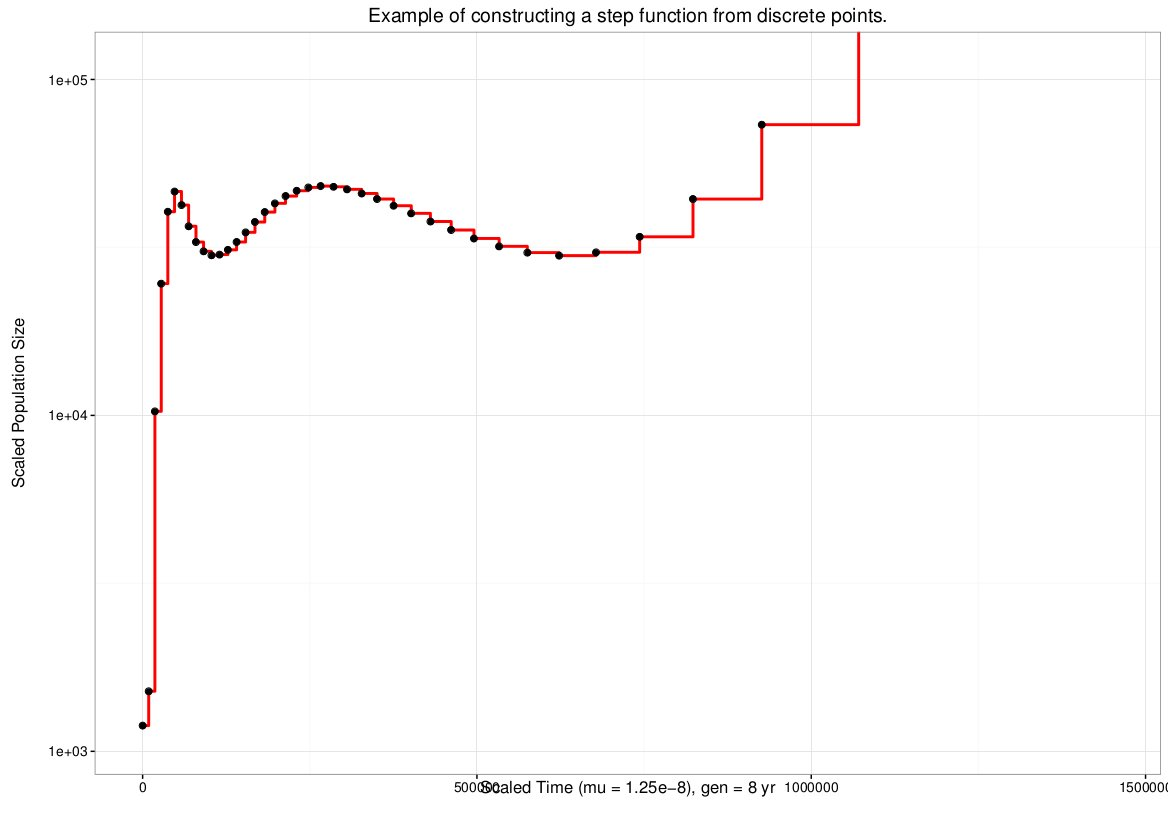
\includegraphics[width=1\textwidth]{pix/pointsToStep}
\caption{The function \texttt{eval\_popsize} allows us to construct a step function (red) from discrete points (black).} \label{pointsToStep}
\end{figure}

The function \texttt{absdifference(xpos,d1,d2,d3,d4)} returns the absolute difference between two MSMC stepwise constant functions $A$ and $B$, evaluated at point \texttt{xpos}. The other inputs to this function are \texttt{d1} and \texttt{d2} (vectors of $\{t_i\}$ and $\{N_e(t_i)\}$ respectively, for $A$), and \texttt{d3} and \texttt{d4} (vectors of $\{t_i\}$ and $\{N_e(t_i)\}$ respectively, for $B$). \texttt{absdifference} uses the \texttt{eval\_popsize} function.

One could then use R's integration function on \texttt{absdifference} to compute the integral that defines the error rate (Equation \ref{errorRate}).

Note that for a population model that involves curves (e.g. exponential growth), the \texttt{absdifference} function may not be so useful. It might be better to write a new \texttt{absdifference} function which takes a MSMC stepwise constant function $A$ as one input, and a curve function $B$ as the other.

\section{Other Suggestions}
\subsection{Reduction In Complexity}
Julien suggested that we could do some trials to see if we recover the same dynamics with say 5 chromosomes, instead of the full 23. This would significantly decrease the run-time of the whole progress. However, fragmenting 5 chromosomes may be quite different to fragmenting 23 chromosomes.


\bibliographystyle{plain}
\bibliography{../references/references}{}

\end{document}
